% !TeX root = ../../thesis.tex
\chapter{Enhancing Photodiode Performance Through Tailored Engineering of the Electron Transport Layer}\label{ch:transport_layer}


Write something about the introduction...


\section{Benchmarking Photodiode Performance}

Building upon prior work conducted within the group, the first step for evaluating the use of the evaporated \ch{CsPbI_2Br} thin films as a photodiode's active layer was to develop a stack that employed DC sputtered \ch{NiO_x} as the HTL and e-beam evaporated \ch{TiO_2} as the ETL \cite{PintorMonroy2021All-EvaporatedApplications}. A unique characteristic of the new composition was the possibility to acquire the $\gamma-$phase without the need of a post-deposition annealing step, therefore, it was highly relevant to compare the PePD performance of two variations: one utilizing an as-deposited perovskite and the other incorporating a flash-annealed perovskite at 300°C in a \ch{N_2} environment. The relevant results are presented in Fig.~\ref{fig:ETL_opt:annealing_impact}a-c. Results indicate that the flash annealed devices exhibit only slightly lower levels of $J_d$ at -2 V (median values are equal 9.5 and 6 $\mu A/cm^2$ for the as-deposited and annealed perovskite, respectively), while their EQE is almost identical, already saturated at 0 V and above 70\% for the most of the visible light spectrum. 

These results emphasize that, despite the improvements in film quality achieved through annealing, as described in Chapter~\ref{ch:ellipsometry} (including improvements in crystalline quality and reduction of non-radiative recombination pathways), its influence on the high-level PePD performance is not as strong. This could be a promising finding for alternative applications that require low-temperature processing of perovskite thin films, such as deposition on flexible substrates, where the as-deposited \ch{CsPbI_2Br} thin films could be employed. For the rest of the presented results, a flash annealing of the perovskite layer at 300 \degree C in \ch{N_2} is always performed before the deposition of the ETL. 

\begin{figure}[htbp]
    \centering
    % First row
    \begin{subfigure}[t]{0.32\textwidth}
        \centering
        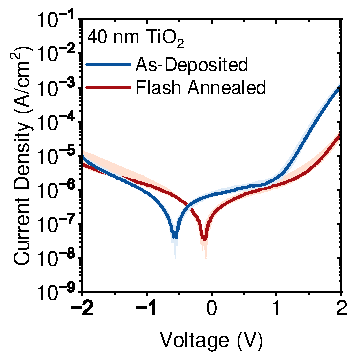
\includegraphics[width=\textwidth]{chapters/material_properties/images/TiO2-Compare.pdf} 
        \caption{}
        \label{fig:ch2:tio2_compare}
    \end{subfigure}
    \hfill
    \begin{subfigure}[t]{0.32\textwidth}
        \centering
        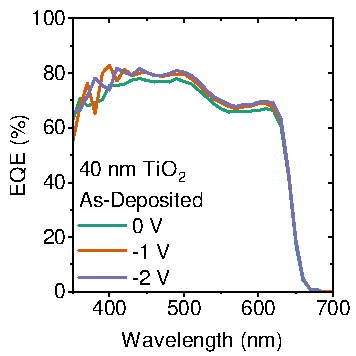
\includegraphics[width=\textwidth]{chapters/material_properties/images/As_Dep-EQE.pdf} % Replace with your image file
        \caption{}
        \label{fig:ch2:as_dep_eqe}
    \end{subfigure}
    \hfill
    \begin{subfigure}[t]{0.32\textwidth}
        \centering
        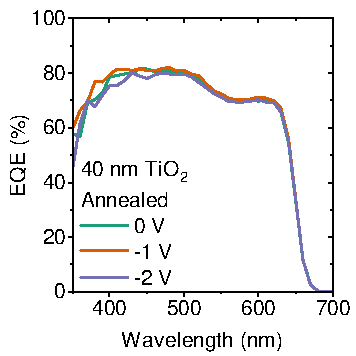
\includegraphics[width=\textwidth]{chapters/material_properties/images/Annealed_EQE.pdf} % Replace with your image file
        \caption{}
        \label{fig:ch2:annealed_eqe}
    \end{subfigure}
    \caption{Impact of annealing on PePD performance.}
    \label{fig:ETL_opt:annealing_impact}
\end{figure}

To further investigate the impact of the perovskite layer deposition and processing conditions on the PePD performance, we pursued two additional variations, one of the \ch{CsBr}:\ch{PbI_2} molar ratio and another of the total deposition rate. The respective results, displaying the variation of $J_d$ and $J_{photo}$ at -2 V for each condition, are shown in Fig.~\ref{fig:etl_opt:molar_and_rate}a and Fig.~\ref{fig:etl_opt:molar_and_rate}b, respectively. It is reminded that the baseline perovskite deposition conditions, rely on the use of a nominal \ch{CsBr}:\ch{PbI_2} ratio equal to 1.05:1.0 and a total deposition rate of 0.8 \AA/s. 

In terms of varying the precursor molar ratio, we explored two additional compositions with \ch{PbI_2} and \ch{CsBr} excess (\ch{CsBr}:\ch{PbI_2} equal to 0.8:1.0 and 1.2:1.0, respectively). The median $J_{photo}$ at -2 V was approximately equal to 13 $\mu A/cm^2$ for all compositions, while the median $J_d$ varied between 5.5 and 16 $\mu A/cm^2$. The 1.05:1.0 composition displayed the optical combination of $J_d$ levels and device variability, even though increasing the amount of CsBr in the film seemed to have a positive effect on the median $J_d$ response. Nevertheless, the difference in performance among devices with different stoichiometry remains relatively small, highlighting the defect tolerance of the perovskite thin films. This means that deviations from the 1.0:1.0 stoichiometry and consequent formation of defects or vacancies does not necessarily lead to increased levels of dark current. Therefore, the potential defect states likely have shallow energy levels that do not promote trap-assisted charge carrier generation in dark conditions.

\begin{figure}[htbp]
    \centering
    
    % Second row
    \begin{subfigure}[t]{0.45\textwidth}
        \centering
        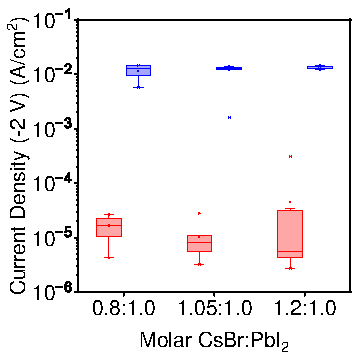
\includegraphics[width=\textwidth]{chapters/transport_layers/images/JV_Box_Ratio.pdf} % Replace with your image file
        \caption{}
        \label{fig:etl_opt:molar_ratio}
    \end{subfigure}
    \hfill
        \begin{subfigure}[t]{0.45\textwidth}
        \centering
        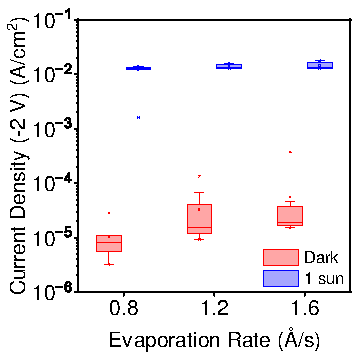
\includegraphics[width=\textwidth]{chapters/transport_layers/images/Evap_Rate_Box_Plot.pdf} % Replace with your image file
        \caption{}
        \label{fig:etl:opt:evap_rate}
    \end{subfigure}    
    \caption{Impact of perovskite deposition parameters on device performance.}
    \label{fig:etl_opt:molar_and_rate}
\end{figure}


For the evaluation of the impact of the total evaporation rate, the nominal 1.05:1.0 \ch{CsBr}:\ch{PbI_2} ratio was maintained, with the evaporation rate being varied from 0.8 to 1.6 \AA/s. Again, the median $J_{photo}$ at -2 V was approximately equal to 13 $\mu A/cm^2$, while the median $J_d$ increased from 8 to 19 $\mu A/cm^2$ as the evaporation rate rose from 0.8 to 1.6 \AA/s. The evaporation rate, along with the substrate temperature, is one of the most critical parameters for the nucleation of the perovskite thin film, as described by equation: 

\begin{equation}
    N \propto \frac{F^p}{D^q}, 
\end{equation}

where N is nuclear density, F is the evaporation rate, and D is the surface diffusion coefficient \cite{Dong2023GrowthFilm}. The values $p$ and $q$ are positive and depend on the nucleation and growth mechanisms. As a result, higher evaporation rates are typically associated with the attainment of smaller grain sizes \cite{Dong2023GrowthFilm, Du2022ThermalOutlook, Shin2020ModulationDiodes}. In a study related to vacuum-deposited \ch{CsPbBr_3} light emitting diodes, Shin et al. identified that by increasing the co-evaporation rate (from 0.4 to 0.9 \AA/s) the grain size was decreased from 100-400 nm to a few tens of nanometers, followed by an enlargement of the exciton binding energy. This tuning led to the development of devices with higher luminance and current efficiency \cite{Shin2020ModulationDiodes}. On the other hand, in a study related to the development of \ch{CsPbI_3}-based solar cells, Dong et al. identified that decreasing the deposition rate did indeed lead to an increase of the average grain size, without though benefiting film crystallization and absorption ability \cite{Dong2023GrowthFilm}. As a result, the rule of thumb that was previously presented, claiming that thermally evaporated solar cells and photodetectors benefit from low deposition rates (and large grain sizes), while thermally evaporated LEDs benefit from high deposition rates (and smaller grain sizes) might be too simplistic without fully considering the complex kinetic dynamics and crystallization mechanisms \cite{Du2022ThermalOutlook}. In the case of our devices, there indeed seems to be a trend where increasing the deposition rate leads to an increase of the $J_d$, however it would not be possible to attribute this effect to a potential decrease of the grain size, especially considering the similar performance of the as-deposited and annealed device in Fig.~\ref{fig:ETL_opt:annealing_impact}. Nevertheless, considering that the use of 0.8 \AA/s yielded the lowest levels of $J_d$, it is the deposition rate used for the rest of the presented results. 


\begin{figure}[htbp]
    \centering
    % Second row
    \begin{subfigure}[t]{0.5\textwidth}
        \centering
        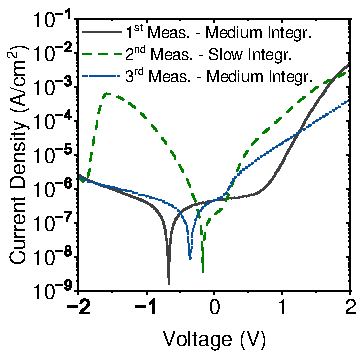
\includegraphics[width=\textwidth]{chapters/transport_layers/images/JV_TiO12_Scan_Speed.pdf} % Replace with your image file
                
    \end{subfigure}

    \caption{Impact of scan speed}
    \label{fig:tio2:scan_speed}
\end{figure}

The results presented thus far provide an initial benchmark for PePD performance and examine the impact of various perovskite-processing parameters. While minor variations are observed, particularly in the $J_d$ level, the impact of these parameters is rather low, highlighting the overall high quality and defect tolerance of the \ch{CsPbI_2Br} thin films. However, an interesting feature comes across when trying to characterize the PePD performance in dark conditions using different integration times. There results are presented in Fig.~\ref{fig:tio2:scan_speed}, where the standard J-V scan with medium integration time is followed by a scan with slow integration time. Even though both measurements start from similar $J_d$ levels, the scan with slow integration time displays an abrupt, almost 3-order of magnitude, increase in the $J_d$ levels while still in the reverse bias regime. The reversibility of this phenomenon is indicated by repeating the J-V scan with medium integration time, where the original performance is recovered. This pattern indicates the triggering of a reverse-bias soft breakdown mechanism, which depends not only on the magnitude of the applied reverse bias, but also its duration \cite{Bertoluzzi2021IncorporatingBias}. Such phenomena have previously been studied in the context of shaded perovskite solar cells, which must carry the current generated by adjacent illuminated cells \cite{Jiang2024ImprovedElectrodes, Ren2024MobileCells, Li2024BarrierBias,Gould2021In-OperandoBias,Razera2020Instability,Bertoluzzi2021IncorporatingBias,Wang2023PerovskiteDegradation,Bowring2018ReverseCells, Ni2021EvolutionIllumination}. Specifically, it was shown that under reverse bias ions accumulate at the perovskite/ETL interface, facilitating the tunneling of holes into the perovskite bulk due to increased band-bending. Recombination centers are thereafter generated by the oxidation of halides to natural halogens \cite{Bertoluzzi2021IncorporatingBias}. Diffusion of iodine into the fullerene-based ETL was also shown to be an aftermath of reverse biasing \cite{Razera2020Instability}. Various breakdown mitigation were proposed, including the introduction of a hole-blocking layer at the perovskite/ETL interface, the use of electrochemically inert electrodes, as well as the deposition thick planarizing polymer HTL. However, reverse-bias breakdown has not been considered in the context of PePDs, where reverse biasing is the standard operating condition. The following section provides a detailed analysis of the reverse-bias breakdown in our vacuum-deposited, all-inorganic PePDs, with a particular focus on the influence of the ETL/perovskite interface quality.


\section{Impact of Perovskite/ETL Interface Quality on Reverse Bias Stability}

\begin{figure}[htbp]
    \centering
    \begin{subfigure}{0.24\textwidth}
        \centering
        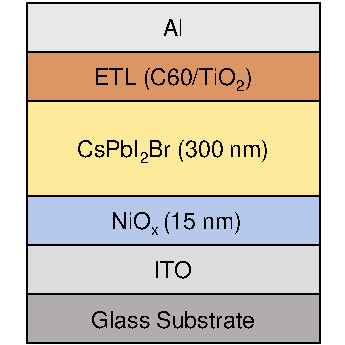
\includegraphics[width=\textwidth]{chapters/transport_layers/images/ETL_optimization_stack.pdf}
        \caption{}
        \label{}
    \end{subfigure}
    \hfill
    \begin{subfigure}{0.24\textwidth}
        \centering
        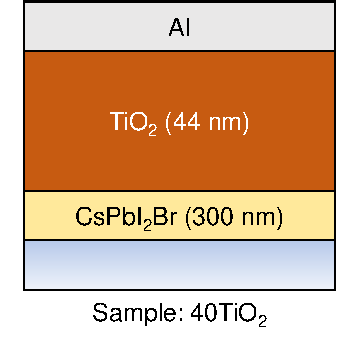
\includegraphics[width=\textwidth]{chapters/transport_layers/images/ETL_Optimization_40TiO2.pdf}
        \caption{}
        \label{}
    \end{subfigure}
    \hfill
    \begin{subfigure}{0.24\textwidth}
        \centering
        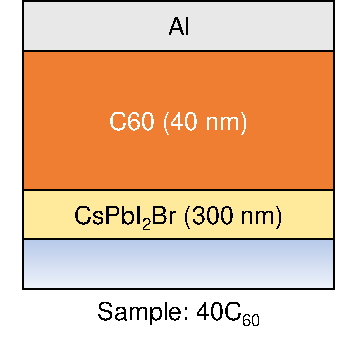
\includegraphics[width=\textwidth]{chapters/transport_layers/images/ETL_Optimization_40C60.pdf}
        \caption{}
        \label{}
    \end{subfigure}
    \hfill
    \begin{subfigure}{0.24\textwidth}
        \centering
        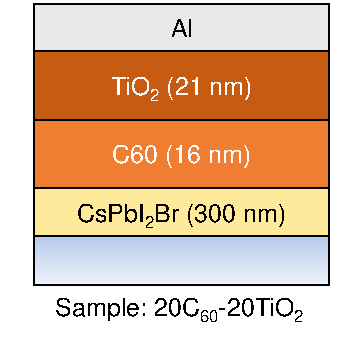
\includegraphics[width=\textwidth]{chapters/transport_layers/images/ETL_Optimization_20_20.pdf}
        \caption{}
        \label{}
    \end{subfigure}
    
    \caption{A 1×4 grid of images.}
    \label{fig:etl_optimization:stacks}
\end{figure}

Considering the importance of the ETL choice on the reverse-bias stability of perovskite-based diodes, we fabricated three variation of the same stack, employing 40 nm of \ch{TiO_2} (Sample 40\ch{TiO_2}), 40 nm of \ch{C_{60}} (Sample 40\ch{C_{60}}), and a 40 nm of a \ch{C_{60}}-\ch{TiO_2} bilayer (Sample 20\ch{C_{60}}-20\ch{TiO_2}) as the device's ETL, as shown in Fig.~\ref{fig:etl_optimization:stacks}a-d. Fig.~\ref{fig:etl_optimization:eds_tem_crossection}a and b displays the STEM-HAADF cross-section of the 40\ch{TiO_2} and 40\ch{C_{60}} samples, respectively, superimposed with their EDS elemental mapping. All layers are continuous and dense, with no visible pinholes, cracks or defects. 


\begin{figure}[htbp]
    \centering
    % First plot
    \begin{subfigure}[t]{0.45\textwidth} % Adjust width as needed
        \centering
        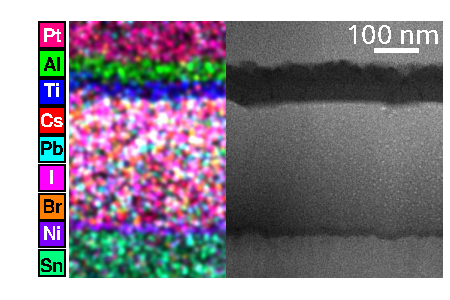
\includegraphics[width=\textwidth]{chapters/transport_layers/images/EDS_TEM_TiO2.pdf} % Replace with your image
        \caption{}
        \label{}
    \end{subfigure}
    \hfill % Space between the two plots
    % Second plot
    \begin{subfigure}[t]{0.45\textwidth} % Adjust width as needed
        \centering
        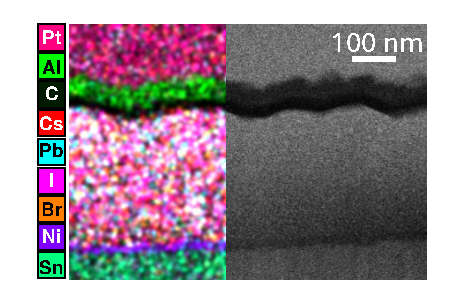
\includegraphics[width=\textwidth]{chapters/transport_layers/images/EDS_TEM_C60.pdf} % Replace with your image
        \caption{}
        \label{}
    \end{subfigure}
    % Caption for the whole figure
    \caption{EDS-TEM Cross-section.}
    \label{fig:etl_optimization:eds_tem_crossection}
\end{figure}

Fig.~\ref{fig:etl_opt:dynamicjv_eqe_staticjv}a-i provide a complete overview of the PePD performance for the three stack variations. Specifically, Fig.~\ref{fig:etl_opt:dynamicjv_eqe_staticjv}a-c show the dynamic J-V scan in darkness and under 1 sun illumination, Fig.~\ref{fig:etl_opt:dynamicjv_eqe_staticjv}d-f show the spectral EQE response of a single device, and lastly Fig.~\ref{fig:etl_opt:dynamicjv_eqe_staticjv}g-i show the static $J_d$ measurements as function of time for increasing reverse bias steps. After each measurement, each device was given an additional 300 seconds to reset in dark. Fig.~\ref{fig:etl_opt:dynamicjv_eqe_staticjv}g highlights the sensitivity of 40\ch{TiO_2} sample to reverse bias breakdown, which is not  hinted by the dynamic scan of Fig.~\ref{fig:etl_opt:dynamicjv_eqe_staticjv}a. In more detail, $J_d$ is maintained below 0.1 $\mu A/cm_2$ after the end of the static scan at -0.5 and -1 V, however, a 3-order of magnitude increase is observed once the bias is increased to -2 V. Even though the primary goal of the work presented in this thesis targets imager applications, where the sub-ms biasing might not be sufficient for the manifestation of the $J_d$ increase, this bias sensitivity could be detrimental for alternative applications that require extensive reverse biasing. Additionally, besides the practical impact on the targeted application, the manifestation of the breakdown mechanism indicates the existence of a defective stack that might impact device performance in non-predicted ways. As a result, it is crucial that it is further understood and addressed. 


\begin{figure}[!ht]
    \centering

    % First row
    \begin{subfigure}[b]{0.32\textwidth}
        \centering
        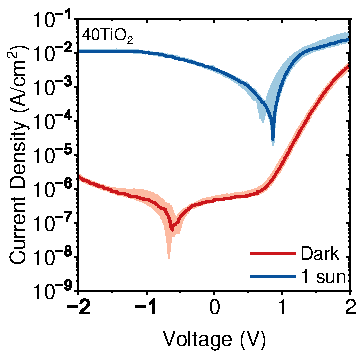
\includegraphics[width=\textwidth]{chapters/transport_layers/images/JV_Median_40TiO2.pdf}
        \caption{}
    \end{subfigure}
    \hfill
    \begin{subfigure}[b]{0.32\textwidth}
        \centering
        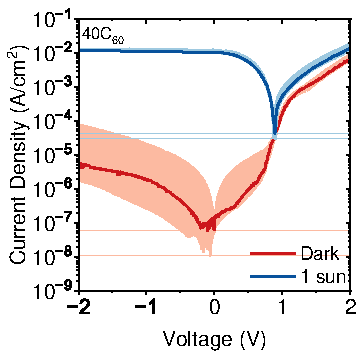
\includegraphics[width=\textwidth]{chapters/transport_layers/images/JV_Median_40C60.pdf}
        \caption{}
    \end{subfigure}
    \hfill
    \begin{subfigure}[b]{0.32\textwidth}
        \centering
        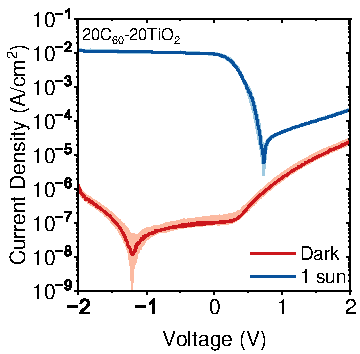
\includegraphics[width=\textwidth]{chapters/transport_layers/images/JV_Median_20_20.pdf}
        \caption{}
    \end{subfigure}


        \begin{subfigure}{0.32\textwidth}
        \centering
        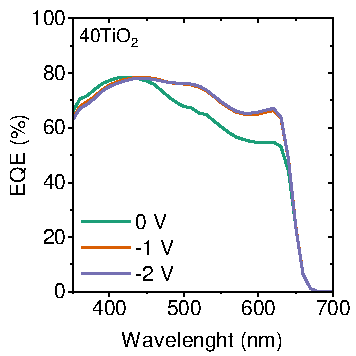
\includegraphics[width=\textwidth]{chapters/transport_layers/images/EQE_40TiO2.pdf}
        \caption{}
        \label{}
    \end{subfigure}
    \hfill
    \begin{subfigure}{0.32\textwidth}
        \centering
        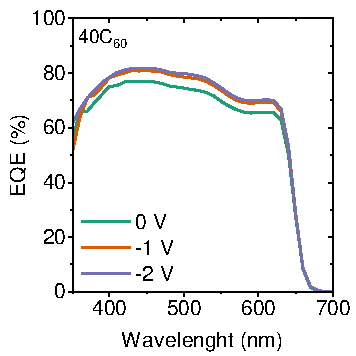
\includegraphics[width=\textwidth]{chapters/transport_layers/images/EQE_40C60.pdf}
        \caption{}
        \label{}
    \end{subfigure}
    \hfill
    \begin{subfigure}{0.32\textwidth}
        \centering
        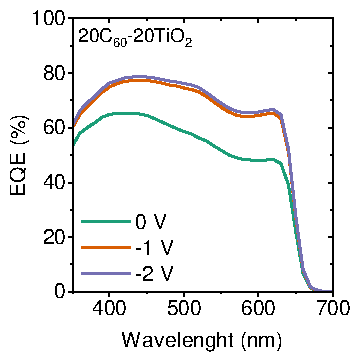
\includegraphics[width=\textwidth]{chapters/transport_layers/images/EQE_20_20.pdf}
        \caption{}
        \label{}
    \end{subfigure}

    % Second row
    \begin{subfigure}[b]{0.32\textwidth}
        \centering
        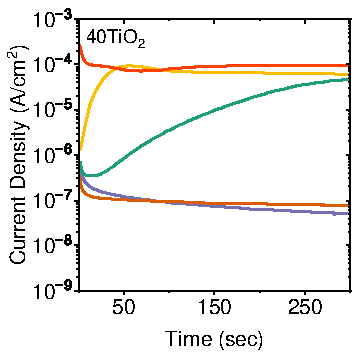
\includegraphics[width=\textwidth]{chapters/transport_layers/images/StaticJV_40TiO2.pdf}
        \caption{}
    \end{subfigure}
    \hfill
    \begin{subfigure}[b]{0.32\textwidth}
        \centering
        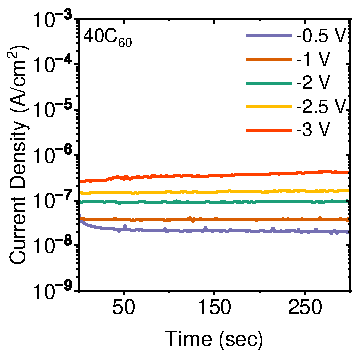
\includegraphics[width=\textwidth]{chapters/transport_layers/images/StaticJV_40C60.pdf}
        \caption{}
    \end{subfigure}
    \hfill
    \begin{subfigure}[b]{0.32\textwidth}
        \centering
        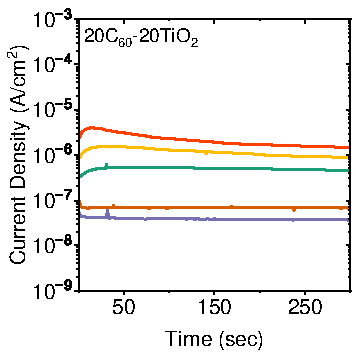
\includegraphics[width=\textwidth]{chapters/transport_layers/images/StaticJV_20_20.pdf}
        \caption{}
    \end{subfigure}

    \caption{A figure with 2 rows and 3 images in each row.}
    \label{fig:etl_opt:dynamicjv_eqe_staticjv}
\end{figure}

In contrary to Sample 40\ch{TiO_2}, the static $J_d$ scan of Sample 40\ch{C_{60}} (Fig.~\ref{fig:etl_opt:dynamicjv_eqe_staticjv}h) shows an almost linear increase of $J_d$ as a function of applied reverse bias, with no indications of breaking down up to -3 V. This result further strengthens the assumption that the perovskite/ETL interface is one of the most critical factors for the reverse bias stability of a PePD. Despite the improved bias stability, Sample 40\ch{C_{60}} is also associated with a large variability in device performance, as indicated by the spread of the interquartile range in Fig.~\ref{fig:etl_opt:dynamicjv_eqe_staticjv}b. The fact that this variability is only observed for the 40\ch{C_{60}} sample is likely due to the incomplete coverage of the perovskite film by the \ch{C_{60}} layer, which leads to the formation of contact pathways between the metal conductor and the perovskite layer \cite{Lin2015LowImaging, Younes2021EnhancingLayer}. This phenomenon seems to be aggravated by the perovskite's small grains size and amount of grain boundaries, as indicated by the comparison of J-V performance of a PePD that employs an as-deposited and flash annealed \ch{CsPbI_2Br} thin film in Fig.~\ref{fig:et_optim:c60_variability_and_1hr_stability}a). Specifically, both the median $J_d$ and the interquartile range show improvement with annealing of the perovskite layer. Nevertheless, the variability of the annealed 40\ch{C_{60}} sample is still significant and unsuitable for a reliable PePD. 


Considering that \ch{C_{60}} is preventing the reverse bias breakdown of the PePD and the use of \ch{TiO_2} ensures higher performance repeatability, the use of a \ch{C_{60}}-\ch{TiO_2} bilayer (of 20 nm each) effectively secures both advantages, as revealed in Fig.~\ref{fig:etl_opt:dynamicjv_eqe_staticjv}c and i. Specifically, $J_d$ remains below 0.5 $\mu A/cm^2$ when the device is biased at -2 V for 300 s and below 2 $\mu A/cm^2$ when biased at -3 V for the same duration. Additionally, there are no signs of breakdown even when biasing the device for 60 minutes at -2 V (Fig.~\ref{fig:et_optim:c60_variability_and_1hr_stability}b). Finally, even though a slight lower EQE at 0 V is observed compared to the 40\ch{TiO_2} and 40\ch{C_{60}} samples (Fig.~\ref{fig:etl_opt:dynamicjv_eqe_staticjv}f), a saturated efficiency above 70\% across the entire visible range is attained for -1 and -2 V. 


\begin{figure}[htbp]
    \centering
    % First plot
    \begin{subfigure}[t]{0.4\textwidth} % Adjust width as needed
        \centering
        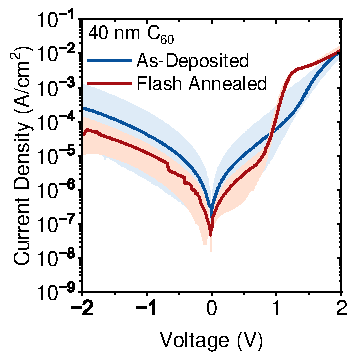
\includegraphics[width=\textwidth]{chapters/material_properties/images/C60-Compare.pdf} % Replace with your image
        \caption{}
        \label{}
    \end{subfigure}
    \hfill % Space between the two plots
    % Second plot
    \begin{subfigure}[t]{0.45\textwidth} % Adjust width as needed
        \centering
        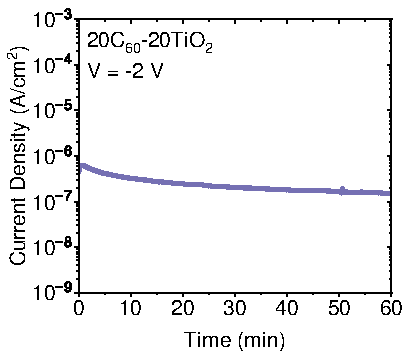
\includegraphics[width=\textwidth]{chapters/transport_layers/images/JV_1hr_20_20.pdf} % Replace with your image
        \caption{}        
        \label{}
    \end{subfigure}

    % Caption for the whole figure
    \caption{Reversibility and long bias}   \label{fig:et_optim:c60_variability_and_1hr_stability}
\end{figure}

Apart from the $J_d$ stability under the effect of reverse bias, evaluating the stability of the PePD's photo-response is as critical, considering that a common concern with perovskite-based solar cells is the loss of power conversion efficiency under continuous illumination \cite{Song2022CriticalAdditives, Fu2019I2Conditions,Khadka2021InsightsJunction}. To investigate this we monitored the EQE of samples 40\ch{TiO_{2}}, 40\ch{C_{60}}, and 20\ch{C_{60}}-20\ch{TiO_2} over time, applying consecutive reverse bias steps and using two different light wavelengths (430 and 620 nm). Given that the samples are illuminated from the glass side, the absorption length of blue (430 nm) and red (620 nm) light are anticipated to correspond to the the HTL/perovskite and perovskite/ETL interface, respectively. Fig.~\ref{fig:etl_opt:static_eqe} provides a summary of the results. At 0 V, samples 40\ch{TiO_2} and 20\ch{C_{60}}-20\ch{TiO_2} display an EQE decrease when illuminated with the 620 nm light source, which however is eliminated when increasing the reverse bias to -1 V. The EQE response at -2 V as a function of time is stable even for sample 40\ch{TiO_2}, which should already be undergoing a breakdown. This indicates that the breakdown current, which is generated and saturated by the recombination of electrons and holes that are injected form the HTL and ETL side, respectively, does not hinder the extraction of photo generated carriers. Besides, as revealed in Fig.~\ref{fig:etl_opt:dynamicjv_eqe_staticjv}, the breakdown current is still two orders of magnitude lower compared to $J_{photo}$ at -2 v. Consequently, the device's specific detective (D*) will be mainly defined by the stability of $J_d$ under reverse bias, rather than the photoresponse. For example, despite having similar EQE response under 620 nm illumination after 300 s at -2 V, sample 40\ch{TiO_2} would have one-order-of-magnitude lower D* compared to 20\ch{C_{60}}-20\ch{TiO_2} (equal to $8.8\times 10^{10}$ and  $8.8\times 10^{11}$ Jones, respectively). 


\begin{figure}[htbp]
    \centering
    \begin{subfigure}{0.32\textwidth}
        \centering
        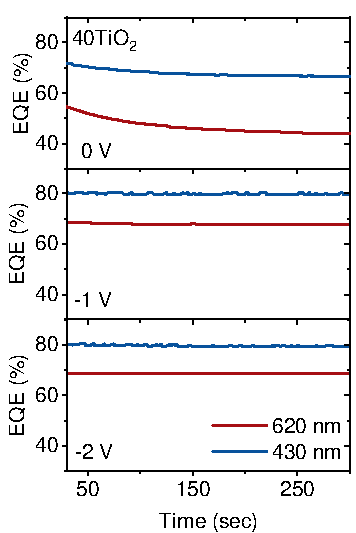
\includegraphics[width=\textwidth]{chapters/transport_layers/images/StaticEQE_40TiO2.pdf}
        \caption{}
        \label{}
    \end{subfigure}
    \hfill
    \begin{subfigure}{0.32\textwidth}
        \centering
        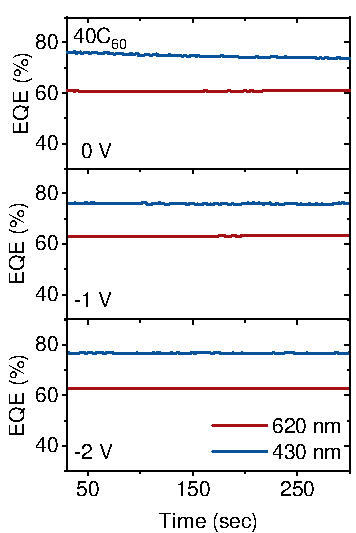
\includegraphics[width=\textwidth]{chapters/transport_layers/images/StaticEQE_40C60.pdf}
        \caption{}
        \label{}
    \end{subfigure}
    \hfill
    \begin{subfigure}{0.32\textwidth}
        \centering
        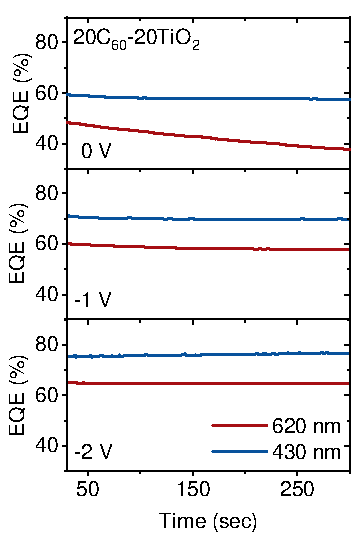
\includegraphics[width=\textwidth]{chapters/transport_layers/images/StaticEQE_20_20.pdf}
        \caption{}
        \label{}
    \end{subfigure}
    
    \caption{A 1×3 grid of images.}
    \label{fig:etl_opt:static_eqe}
\end{figure}

With the results presented so far, it is clear that the deposition of 20 nm of \ch{C_{60}} between the perovskite and the \ch{TiO_2} layer is critical for the prevention of the PePD's breakdown under the effect of reverse bias. To determine whether a minimum \ch{C_{60}} thickness is required to ensure the device's reverse bias stability, we fabricated a fourth variation of the same stack, incorporating a 10 nm \ch{C_{60}} and a 30 nm \ch{TiO_2} layer as the ETL (sample 10\ch{C_{60}}-30\ch{TiO_2} in Fig.~\ref{fig:etl_opt:10nmC60_30nmTiO2}a). The dynamic and static J-V scan, as well as the device's EQE are shown in Fig.~\ref{fig:etl_opt:10nmC60_30nmTiO2}b-d, with the 3-order-of-magnitude increase of $J_d$ under the effect of -3 V revealing that 10 nm of \ch{C_{60}} are not in fact sufficient to fully protect the perovskite layer.


\begin{figure}[t]
    \centering
    % First row
    \begin{subfigure}[t]{0.4\textwidth}
        \centering
        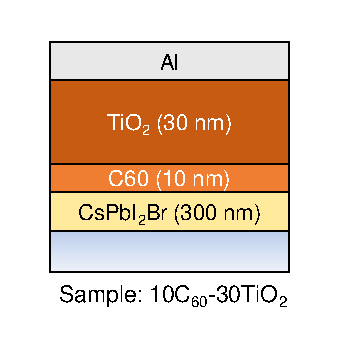
\includegraphics[width=\textwidth]{chapters/transport_layers/images/Sample_10_30_icon.pdf} % Replace with your image file
        \caption{}
        \label{}
    \end{subfigure}
    \hfill
    \begin{subfigure}[t]{0.4\textwidth}
        \centering
        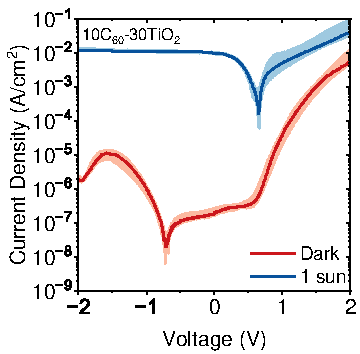
\includegraphics[width=\textwidth]{chapters/transport_layers/images/JV_Median_10_30.pdf} 
        % Replace with your image file
        \caption{}
        \label{}
    \end{subfigure} 
 % Second row
    \begin{subfigure}[t]{0.4\textwidth}
        \centering
        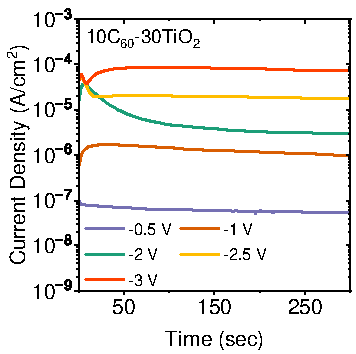
\includegraphics[width=\textwidth]{chapters/transport_layers/images/StaticJV_10_30.pdf} % Replace with your image file
        \caption{}
        \label{}
    \end{subfigure}
    \hfill
    \begin{subfigure}[t]{0.4\textwidth}
        \centering
        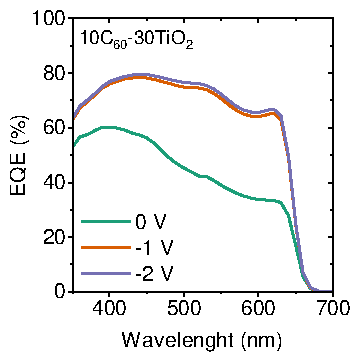
\includegraphics[width=\textwidth]{chapters/transport_layers/images/EQE_10_30.pdf} % Replace with your image file
        \caption{}
        \label{}
    \end{subfigure}
    \caption{}
    \label{fig:etl_opt:10nmC60_30nmTiO2}
\end{figure}


To further investigate the physical origin of the reverse bias instability of the 40\ch{TiO_2} sample as well as the performance variability the 40\ch{C_{60}}, we examine the EDS elemental concentration profiles of the three stacks, which are shown in Fig.~\ref{fig:etl_opt:eds_concentration}a-c. Having as reference the onset of the \ch{Pb} signal, a dashed line is drawn in each plot to indicate the start of the perovskite layer. In contrast to sample 40\ch{C_{60}}, the Cs signal for sample 40\ch{TiO_2} is starting much earlier compared to Pb, I, and Br, pointing out to a significantly altered perovskite stoichiometry at the interface. The significant change in surface stoichiometry of the 40\ch{TiO_2} sample is likely responsible for increased inter-bandgap states, which enhance hole tunneling under reverse bias \cite{Huang2018IntrinsicCsPbI3, Kang2017HighCsPbBr3, Chu2020SoftDefects}. On the other hand, the elemental concentrations of sample 40\ch{C_{60}} reveal an overlapping of the Al signal and perovskite's constituents elements, further supporting the claim for incomplete surface coverage by the \ch{C_60} layer and the creation of metallic shorts that promote performance variability among devices fabricated on the same substrate. Finally, the elemental profile of sample 20\ch{C_{60}}-20\ch{TiO_2} indicates that the bilayer ETL configuration helps preserving the perovskite's surface stoichiometry, reducing the diffusion of Cs in the ETL (albeit not completely eliminating), while at the same time establishing a better separation between the Al contact and the perovskite. 



\begin{figure}[htbp]
    \centering
    \begin{subfigure}{0.32\textwidth}
        \centering
        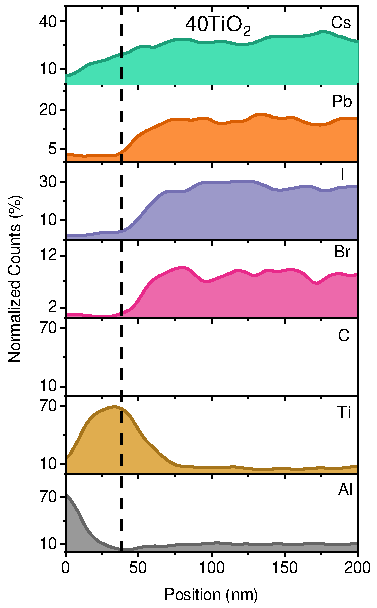
\includegraphics[width=\textwidth]{chapters/transport_layers/images/TEM_40TiO2.pdf}
        \caption{}
        \label{}
    \end{subfigure}
    \hfill
    \begin{subfigure}{0.32\textwidth}
        \centering
        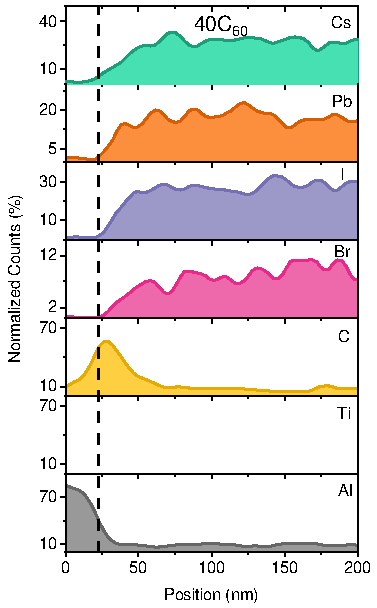
\includegraphics[width=\textwidth]{chapters/transport_layers/images/TEM_40C60.pdf}
        \caption{}
        \label{}
    \end{subfigure}
    \hfill
    \begin{subfigure}{0.32\textwidth}
        \centering
        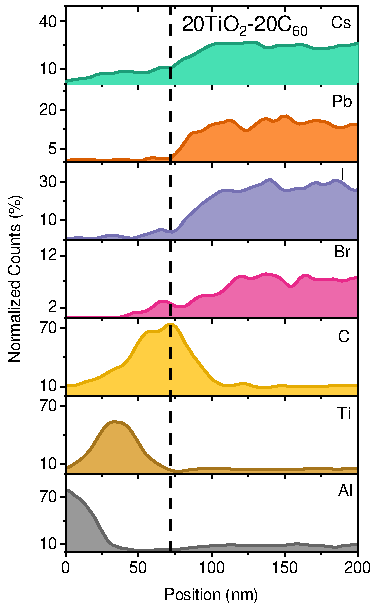
\includegraphics[width=\textwidth]{chapters/transport_layers/images/TEM_20_20.pdf}
        \caption{}
        \label{}
    \end{subfigure}
    
    \caption{A 1×3 grid of images.}
    \label{fig:etl_opt:eds_concentration}
\end{figure}

To further evaluate the perovskite/ETL interface quality we employ transient photocurrent (TPC) measurements, exciting the PePDs with two different light sources, a white and red (625 nm) light one. Their respective spectral profile is shown in Fig.~\ref{fig:etl_opt:tpc_sources_and_simulation}a and b, where the LED irradiance has been tuned to yield a total intensity of 44.5 $mW/cm^2$ and 25.5 $mW/cm^2$ for the white and red light source, respectively. Using different light sources leads to different carrier generation profiles within the perovskite layer, enabling the disentanglement of bulk- and interface-dominated phenomena. The carrier generation rate as a function of distance inside the perovskite layer can be simulated using the optical constants of each device layer (obtained via spectroscopic ellipsometry) as an input in the transfer matrix algorithm \cite{Burkhard2010AccountingCells}. The model developed for the simulation is illustrated in Fig.~\ref{fig:etl_opt:tpc_sources_and_simulation}c, while  the carrier generation rate within the \ch{CsPbI_2Br} layer for both light sources is shown in Fig.~\ref{fig:etl_opt:tpc_sources_and_simulation}d. 


\begin{figure}[t]
    \centering
    % First row
    \begin{subfigure}[t]{0.45\textwidth}
        \centering
        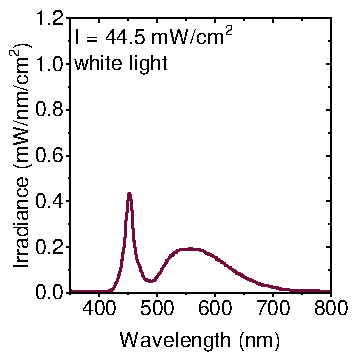
\includegraphics[width=\textwidth]{chapters/transport_layers/images/white_led.pdf} % Replace with your image file
        \caption{}
        \label{}
    \end{subfigure}
    \hfill
    \begin{subfigure}[t]{0.45\textwidth}
        \centering
        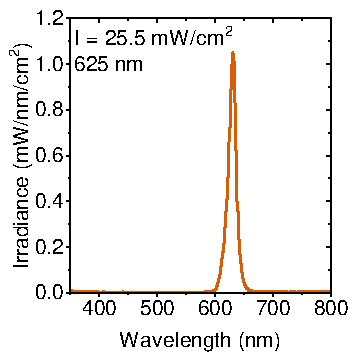
\includegraphics[width=\textwidth]{chapters/transport_layers/images/red_led.pdf} 
        % Replace with your image file
        \caption{}
        \label{}
    \end{subfigure} 
 % Second row
    \begin{subfigure}[t]{0.45\textwidth}
        \centering
        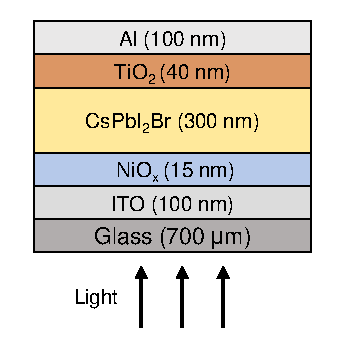
\includegraphics[width=\textwidth]{chapters/transport_layers/images/transfer_matrix_model.pdf} % Replace with your image file
        \caption{}
        \label{}
    \end{subfigure}
    \hfill
    \begin{subfigure}[t]{0.45\textwidth}
        \centering
        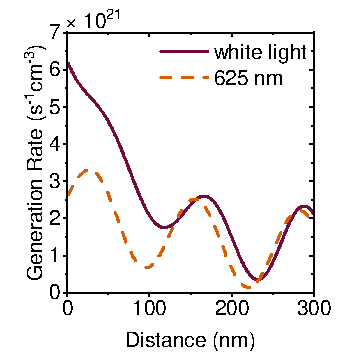
\includegraphics[width=\textwidth]{chapters/transport_layers/images/Generation_Rate.pdf} % Replace with your image file
        \caption{}
        \label{}
    \end{subfigure}
    \caption{}
    \label{fig:etl_opt:tpc_sources_and_simulation}
\end{figure}


A summary of TPC results for all PePDs is provided in Fig.~\ref{fig:etl_opt:tpc_comparison}a-d. For each sample and light source, the TPC response was measured at -1 and -2 V, with all curves normalized relative to the -2 V response. Starting with samples 40\ch{C_{60}} and 20\ch{C_{60}}-20\ch{TiO_2}, the photocurrent response under the effect of -1 and -2 V is similar for both illumination conditions. However, as the \ch{C_{60}} layer thickness decreases, a larger discrepancy under the effect of -1 and -2 V is observed. Specifically, the TPC response under -2 V has a square shape that corresponds to the light pulse that starts at 0 ms. In contrast, with the PePD biased at -1 V, the photocurrent initially rises as a response to the light pulse but begins to decline within a few tens of microseconds, before stabilizing at a lower value for the remainder of the light pulse. This effect is more pronounced under the effect of 625 nm illumination, although sample 40\ch{TiO_2} begins exhibiting this pattern even under white light illumination.


\begin{figure}[htbp]
    \centering
    \begin{subfigure}{0.24\textwidth}
        \centering
        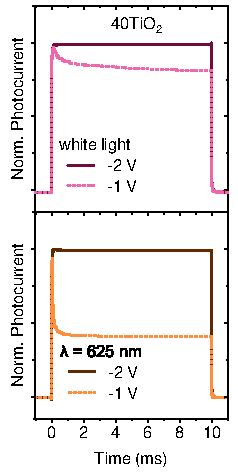
\includegraphics[width=\textwidth]{chapters/transport_layers/images/TPC_40TiO2.pdf}
        \caption{}
        \label{}
    \end{subfigure}
    \hfill
    \begin{subfigure}{0.24\textwidth}
        \centering
        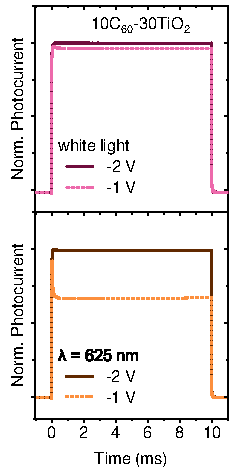
\includegraphics[width=\textwidth]{chapters/transport_layers/images/TPC_10_30.pdf}
        \caption{}
        \label{}
    \end{subfigure}
    \hfill
    \begin{subfigure}{0.24\textwidth}
        \centering
        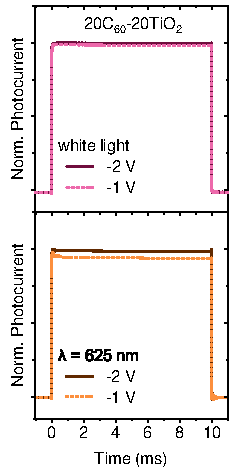
\includegraphics[width=\textwidth]{chapters/transport_layers/images/TPC_20_20.pdf}
        \caption{}
        \label{}
    \end{subfigure}
    \hfill
    \begin{subfigure}{0.24\textwidth}
        \centering
        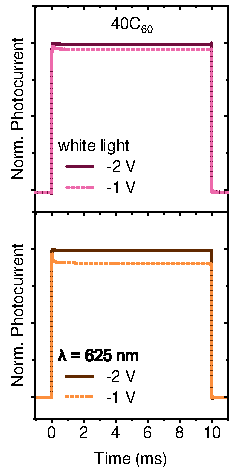
\includegraphics[width=\textwidth]{chapters/transport_layers/images/TPC_40C60.pdf}
        \caption{}
        \label{}
    \end{subfigure}
    
    \caption{A 1×4 grid of images.}
    \label{fig:etl_opt:tpc_comparison}
\end{figure}

Such phenomena of transient peaks in the TPC response of organic- and perovskite-based photodiodes were previously associated with a non-ideal charge extraction and carrier accumulation at an interface \cite{Neophytou2019EnhancingLayer, Hwang2009Drift-diffusionCells,Mcneill2009PhotocurrentEffects}. Specifically, in the presence of a defect-rich interface, in this case the perovskite/ETL interface, electrons may get trapped near the anode, leading to a local reduction of the electric field via the creation of a space-charge region. This in turn limits charge separation and promotes recombination \cite{Mcneill2009PhotocurrentEffects}. The electron trapping rate, and by extension the width of the space charge region, depends of course on the interface's defect density but also the charge generation rate in the same region \cite{Hwang2009Drift-diffusionCells}. However, Fig.~\ref{fig:etl_opt:tpc_sources_and_simulation}d revealed that the charge generation rate at the perovskite/ETL interface (Distance = 300 nm) is similar for both white and red light illumination, and equal to approximately $2\times 10^{21}s^{-1}cm^{-3}$. As a result, and taking as example the 40\ch{TiO_2} sample, we could reasonable consider similar levels of trapped-charge accumulation at the perovskite/ETL interface for both types of illumination, leading to the formation of a space-charge region of similar width. Yet, as shown in Fig.~\ref{fig:etl_opt:tpc_comparison}a, the transient peak is more pronounced under the effect of red light illumination. This is attributed to the fact that under white light illumination a larger percentage of carriers is generated closer to HTL/perovskite interface (Distance = 0 nm in Fig.~\ref{fig:etl_opt:tpc_sources_and_simulation}d), which can be more efficiently separated and extracted, dominating in the sample's TPC response. In conclusion, the diminishing TPC peak under red light illumination and -1 V bias with increasing \ch{C_{60}} layer thickness is further supporting the claim that the reverse bias breakdown is eliminated through a reduction in the density of interface trap states.

Interestingly, the saturated TPC response of sample 40\ch{TiO_2} under 625 nm light illumination at -1 V is almost half compared to -2 V. On the other hand, the saturated EQE response of the same sample at 620 nm (Fig.~\ref{fig:etl_opt:static_eqe}a) is approximately equal to 70\% when the PePD is biased at -1 and -2 V. This discrepancy is attributed to the significantly lower intensity of the EQE light source (<3 $mW/cm^2$ compared to 25.5 $mW/cm^2$) and the fact that the accumulation of trapped charge at the perovskite/ETL interface is directly proportional to it \cite{Hwang2009Drift-diffusionCells,Mcneill2009PhotocurrentEffects}.

\section{Impact of ETL on Response Speed}

\begin{figure}[htbp]
    \centering
    % First row
    \begin{subfigure}[t]{0.4\textwidth}
        \centering
        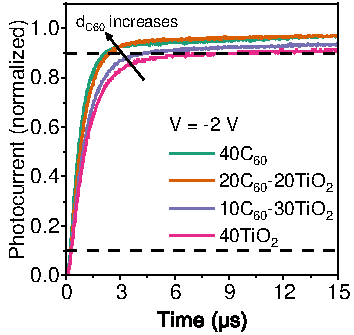
\includegraphics[width=\textwidth]{chapters/transport_layers/images/TPC_comparison_v2.pdf} % Replace with your image file
        \caption{}
        \label{}
    \end{subfigure}
    \hfill
    \begin{subfigure}[t]{0.37\textwidth}
        \centering
        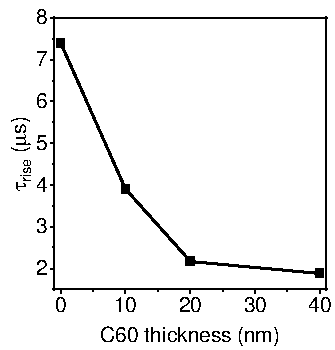
\includegraphics[width=\textwidth]{chapters/transport_layers/images/Rise_time_f_c60_thickness.pdf} 
        % Replace with your image file
        \caption{}
        \label{}
    \end{subfigure} 
 % Second row
    \begin{subfigure}[t]{0.44\textwidth}
        \centering
        \hspace{-1.5cm}
        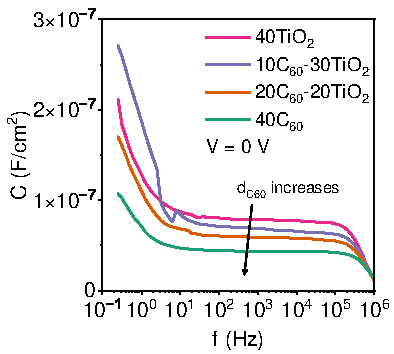
\includegraphics[width=\textwidth]{chapters/transport_layers/images/Cf_comparison.pdf} % Replace with your image file
        \caption{}
        \label{}
    \end{subfigure}
    \hfill
    \begin{subfigure}[t]{0.4\textwidth}
        \centering
        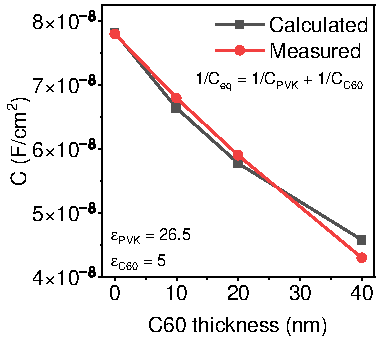
\includegraphics[width=\textwidth]{chapters/transport_layers/images/C_f_c60_thick.pdf} % Replace with your image file
        \caption{}
        \label{}
    \end{subfigure}
    \caption{}
    \label{fig:etl_opt:rise_time_and_capacitance}
\end{figure}

Besides the investigation of the perovskite/ETL interface quality, the TPC measurements can be further used to evaluate the carrier extraction speed of the PePDs, which is defined as the time it takes for the device to respond to the transient light pulse. Fig.~\ref{fig:etl_opt:rise_time_and_capacitance}a superimposes the photoresponse of the four PePDs, biased at -2 V, during the first microseconds of the measurement under white light illumination. A distinct trend emerges, where the response becomes faster as the \ch{C_{60}} layer thickness increases. The PePDs' rise time ($\tau_r$) can be further quantified as the time required for the photocurrent to reach 90\% of its steady-state value (starting from 10\%). Fig.~\ref{fig:etl_opt:rise_time_and_capacitance}b displays the extracted $\tau_r$ as a function of the \ch{C_{60}} layer thickness, highlighting the impact of the chosen ETL configuration on the detector's speed.  

\begin{figure}[htbp]
    \centering
    \begin{subfigure}{0.32\textwidth}
        \centering
        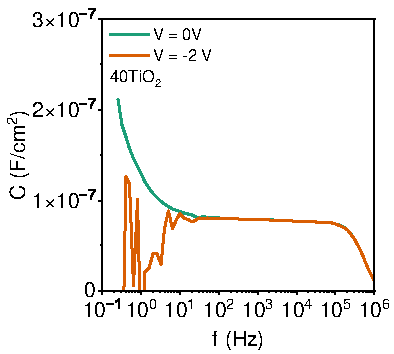
\includegraphics[width=\textwidth]{chapters/transport_layers/images/Cf_40TiO2.pdf}
        \caption{}
        \label{}
    \end{subfigure}
    \hfill
    \begin{subfigure}{0.32\textwidth}
        \centering
        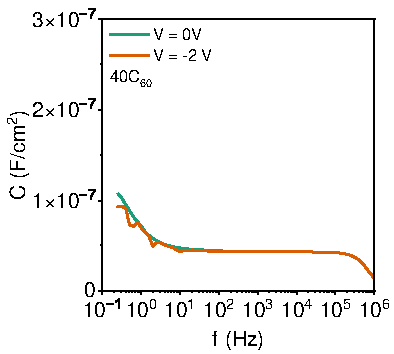
\includegraphics[width=\textwidth]{chapters/transport_layers/images/Cf_40C60.pdf}
        \caption{}
        \label{}
    \end{subfigure}
    \hfill
    \begin{subfigure}{0.32\textwidth}
        \centering
        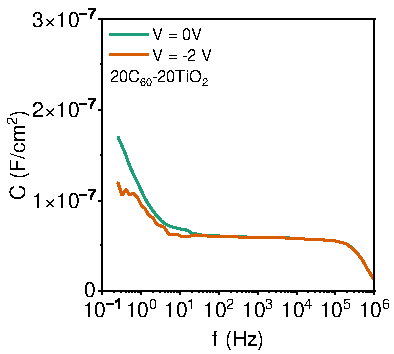
\includegraphics[width=\textwidth]{chapters/transport_layers/images/Cf_20_20.pdf}
        \caption{}
        \label{}
    \end{subfigure}
    
    \caption{A 1×3 grid of images.}
    \label{fig:etl_opt:cf_all}
\end{figure}



Considering that the RC time constant is critical for a photodiode's response speed, we characterize the devices' capacitance as a function of frequency at 0 and -2 V (Fig.~\ref{fig:etl_opt:cf_all}a-c). For frequencies above 10 Hz, samples 40\ch{C_{60}} and 20\ch{C_{60}}-20\ch{TiO_2} have identical capacitance at 0 and -2 V, revealing that the built-in potential is sufficient to fully deplete the PePDs, without the need for additional reverse bias. This further suggests that the increase in the devices' response speed when a thicker \ch{C_{60}} layer is used can not be attributed to an extension of the depletion region within the perovskite layer itself \cite{Goushcha2017OnPhotodiodes}. The signal of the capacitance measurement for sample 40\ch{TiO_2} exhibits the same trend, even though it is collapsing to 0 and becomes more noisy for frequencies below 10 Hz, a direct aftermath of the device breakdown after reverse biasing for prolonged duration. Fig.~\ref{fig:etl_opt:rise_time_and_capacitance}c provides a overlay comparison of the C-f measurement for all PePDs in absence of any external bias. For moderate frequencies, in the range of 10Hz to 100 kHz, the capacitance of the device is inversely proportional to the thickness of the \ch{C_{60}} layer, in agreement with the observed increase in response speed ($\tau_r \propto \tau_{RC}$). Considering that the equivalent device capacitance for a series connection is equal to 
 
 \begin{equation}
    \frac{1}{C_{eq}} = \frac{1}{C_{pvkt}} + \frac{1}{C_{ETL}}
    \label{eg:series_cap}
 \end{equation}

, the decrease in $C_{eq}$ could potentially be attributed to an extension of the depletion width within the \ch{C_{60}} layer, as it was previously numerically shown and attributed to the relatively low doping density of the material \cite{Pham2023EffectsCells}.  

\begin{figure}[htbp]
    \centering
    % First plot
    \begin{subfigure}[t]{0.35\textwidth} % Adjust width as needed
        \centering
        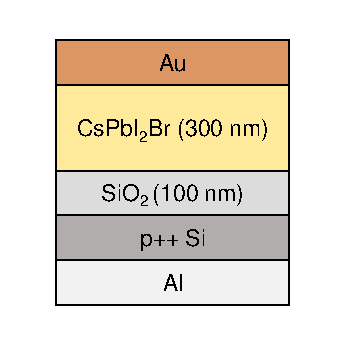
\includegraphics[width=\textwidth]{chapters/transport_layers/images/MOS_Structure_icon.pdf} % Replace with your image
        \caption{}
        \label{}
    \end{subfigure}
    \hfill % Space between the two plots
    % Second plot
    \begin{subfigure}[t]{0.4\textwidth} % Adjust width as needed
        \centering
        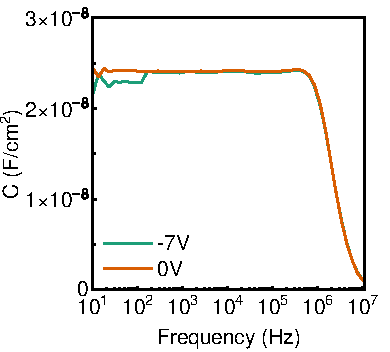
\includegraphics[width=\textwidth]{chapters/transport_layers/images/MOS_IS.pdf} % Replace with your image
        \caption{}
        \label{}
    \end{subfigure}

    % Caption for the whole figure
    \caption{Reversibility and long bias}
    \label{}
\end{figure}


\begin{table}[htbp]
    \centering
    \renewcommand{\arraystretch}{1.5} % Adjust row spacing
    \begin{tabular}{@{} l l @{}}
        \hline
        C [$F/cm^2$] & $7.8\times10^{-8}$\\ \hline
        $\epsilon_0$ [$F/m$]& $8.85\times10^{-12}$ \\ \hline
        $d_{pvkt}$ [$nm$] & $300$ \\ \hline
        A [$cm^2$] & $0.125$ \\ \hline
    \end{tabular}
    \caption{Example Table with Horizontal Lines} % Caption for the table
    \label{tab:etl_opt:er_from_pepd} % Label for referencing
\end{table}

To verify this hypothesis, we first extract perovskite's relative permittivity ($\epsilon_r$) from the C-f of sample 40\ch{TiO_2}, considering that the depletion region is limited within the \ch{CsPbI_2Br} layer and using equation $C_{pvkt} = \frac{\epsilon_r\epsilon_0A}{d}$, where $\epsilon_0$ is the vacuum permittivity, $A$ is the device area and $d$ is the perovskite thickness. Using the values that are summarized in Table~\ref{tab:etl_opt:er_from_pepd}, we extract $\epsilon_r = 26.5$. In order to corroborate this value and eliminate the influence of the ETL, we additionally fabricate a metal-oxide-semiconductor (MOS) capacitor, that employs heavily a p-doped silicon wafer as the metal contact and a thermally-grown \ch{SiO_2} (100 nm) layer as the oxide. The schematic of the MOS-stack, as well as the results of the C-f measurement at 0 and -7 V are shown in Fig.~\ref{tab:etl_opt:er_from_mos}a and b, respectively. Taken into account that the perovskite and oxide are connected in series (eq.~\ref{eg:series_cap}) and using the values of Table~\ref{tab:etl_opt:er_from_mos}, we extract $\epsilon_r = 26.9$, which is in great agreement with the value that was estimated from the 40\ch{TiO_2} sample. Finally, Fig.~\ref{fig:etl_opt:rise_time_and_capacitance}d compares the measured and numerically calculated equivalent capacitance of the PePDs as function of the \ch{C_{60}} layer, considering that the latter is fully depleted. The strong agreement between measured and calculated values further confirms our initial hypothesis that the increase in the PePDs response with increasing \ch{C_{60}} layer thickness is attributed to a reduction of the stack's RC constant, though an extension of the depletion area towards the \ch{C_{60}} layer \cite{Goushcha2017OnPhotodiodes}. 

\begin{table}[htbp]
    \centering
    \renewcommand{\arraystretch}{1.5} % Adjust row spacing
    \begin{tabular}{@{} l l @{}}
        \hline
        $C_{eq}$ [$F/cm^2$] & $2.4\times10^{-8}$\\ \hline
        $\epsilon_0$ [$F/m$]& $8.85\times10^{-12}$ \\ \hline
        $\epsilon_{r,SiO_2}$ & 3.9 \\ \hline
        $d_{SiO_2}$ [$nm$] & $100$ \\ \hline
        $d_{pvkt}$ [$nm$] & $300$ \\ \hline
        A [$cm^2$] & $0.16$ \\ \hline
    \end{tabular}
    \caption{Example Table with Horizontal Lines} % Caption for the table
    \label{tab:etl_opt:er_from_mos} % Label for referencing
\end{table}

This finding gives the motivation of further increasing the c-60 layer thickness to achive even faster detector response....


\begin{figure}[htbp]
    \centering
    \begin{subfigure}{0.35\textwidth}
        \centering
        \includegraphics[width=\textwidth]{chapters/transport_layers/images/Capacitance_f_area.pdf}
        \caption{}
        \label{}
    \end{subfigure}
    \hfill
    \begin{subfigure}{0.3\textwidth}
        \centering
        \includegraphics[width=\textwidth]{chapters/transport_layers/images/TPC_f_area.pdf}
        \caption{}
        \label{}
    \end{subfigure}
    \hfill
    \begin{subfigure}{0.29\textwidth}
        \centering
        \includegraphics[width=\textwidth]{chapters/transport_layers/images/Rise_time_farea.pdf}
        \caption{}
        \label{}
    \end{subfigure}
    
    \caption{A 1×3 grid of images.}
    \label{}
\end{figure}



\section{Conclusions}



%%%%%%%%%%%%%%%%%%%%%%%%%%%%%%%%%%%%%%%%%%%%%%%%%%
% Keep the following \cleardoublepage at the end of this file, 
% otherwise \includeonly includes empty pages.
\cleardoublepage

